\documentclass{article}
% set up the page formatting
\usepackage[a4paper, portrait, margin=2.5cm]{geometry}
\usepackage{multicol}
\usepackage{fancyhdr}
\usepackage{xcolor}
\usepackage{graphicx}
\usepackage{float}

% allow for table of contents clickable links
\usepackage{hyperref}

% editable bits
\title{CS261 Group 29 Planning and Design}
\author{Ani Bitri, Krister Hughes, Thomas Phuong, Eshan Sharif, Josh Turner, Antoni Zyla}
\date{January 2025}
\fancyfoot[L]{Planning and Design}
\fancyfoot[R]{\thepage}

\begin{document}
\maketitle


\section{Team Planning}
\subsection{Time Management}
The Gantt chart below shows the planned work schedule for the project. Team meetings will occur every Wednesday to discuss progress and ensure adherence to the schedule.

\begin{figure}[H]
    \centering
    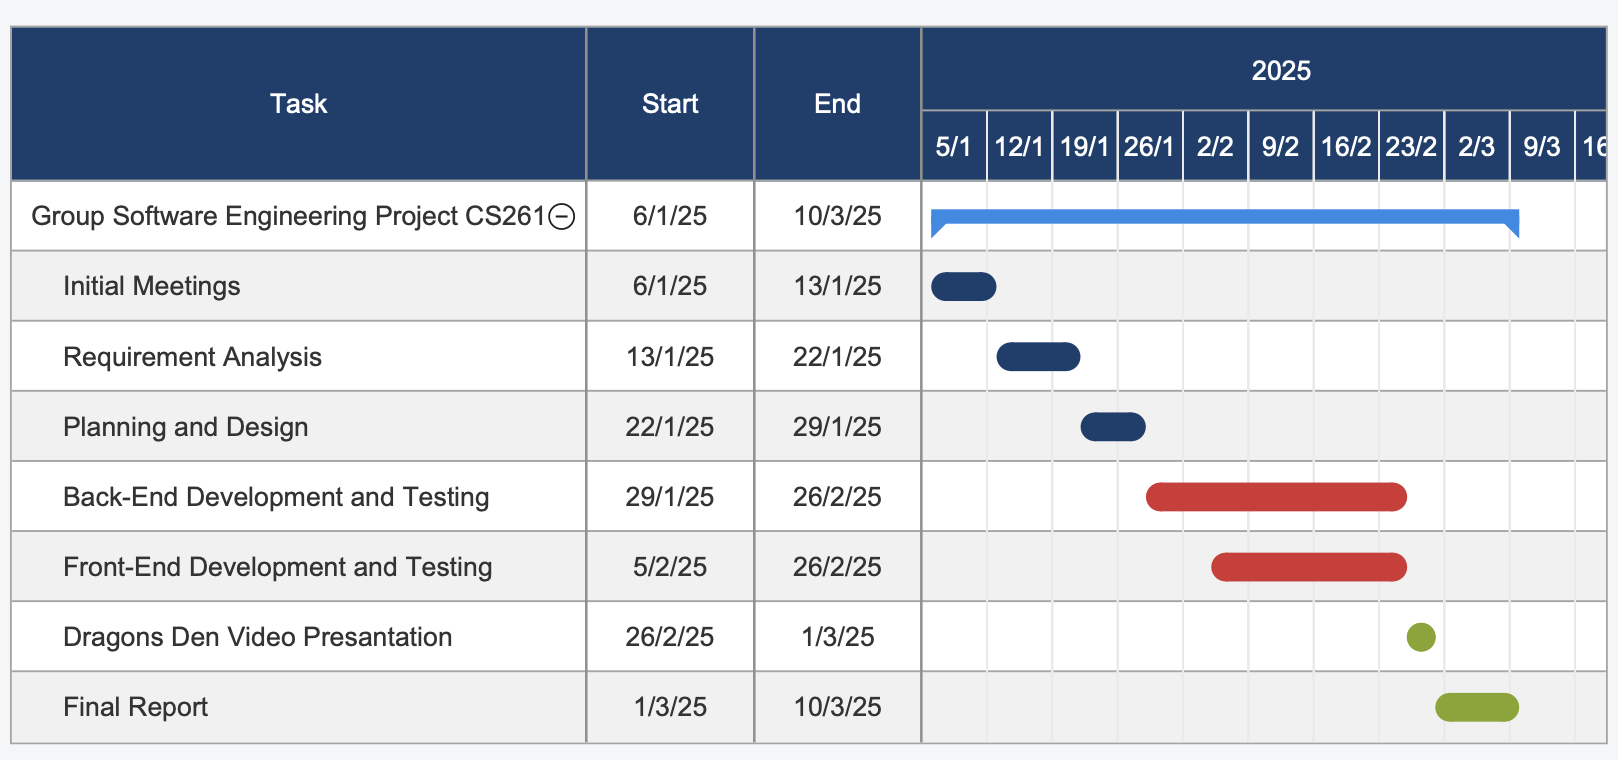
\includegraphics[width=\textwidth]{ganttchart.png}
    \caption{Gantt Chart of Planned Work Schedule}
    \label{fig:gantt_chart}
\end{figure}

\subsection{Software Development Methodology}
For our project, we have chosen to follow a slight variation of the Waterfall Methodology, with the variation 
being the possibility to reevaluate the requirements and design part way through the project, if newer 
requirements are put forward. This variation is included because the client mentioned there was a possibility 
of introducing new requirements some point into the development process. The team agreed to adopt the Waterfall 
Methodology since other than the previously mentioned case, there is no room for significant changes during the 
development. Given the project's well-defined requirements and structured approach, the Waterfall Methodology 
ensures a systematic progression through each phase. Furthermore, other methodologies require frequent communication 
with the client, which the timescale of the project deems it difficult to achieve.

\subsection{Risk Assessment and Management}
We have identified the following risks and have agreed on the following mitigation strategies:
\subsubsection{Technology Limitations}
\begin{itemize}
    \item Risk description: Team/Team members may be unfamiliar to some tool, libraries, or frameworks, which may cause delays or reduced performance. 
    \item Risk Level: \textcolor{green}{Tolerable}
    \item Risk Likelihood: \textcolor{orange}{Moderate}
    \item Mitigation Strategy: Assign tasks to team members based on their expertise in relevant technologies while ensuring everyone is involved in meaningful roles to maintain prductivity and foster teamwork.
\end{itemize}

\subsubsection{Rollback Challenges}
\begin{itemize}
    \item Risk description: Lack of a version control system could prevent from rolling back to the software's last stable state in case of errors
    \item Risk Level: \textcolor{red}{Catastrophic}
    \item Risk Likelihood: \textcolor{green}{Low}
    \item Mitigation Strategy: Utilise github to always maintain a stable version of the software and updating it when being sure that the changes will not affect its usability. 
\end{itemize}

\subsubsection{Testing Risks}
\begin{itemize}
    \item Risk description: Insufficient testing may reduce confidence in the software
    \item Risk Level: \textcolor{orange}{Serious}
    \item Risk Likelihood: \textcolor{orange}{Moderate}
    \item Mitigation Strategy: Unit tests will be designed to test the software to make sure that it is working properly.
\end{itemize}

\subsubsection{Time Management}
\begin{itemize}
    \item Risk description: Underestimating  task duration or improper prioritization might result in delayed work.
    \item Risk Level: \textcolor{orange}{Serious}
    \item Risk Likelihood: \textcolor{green}{Low}
    \item Mitigation Strategy: The team is meeting in regular intervals to ensure work efficiency and mitigate time related risks.
\end{itemize}

\subsubsection{Requirement Misalignment}
\begin{itemize}
    \item Risk description: During the development of the software, the end product might not be the same as the one describe in the deliverables due to unforeseen circumstances
    \item Risk Level: \textcolor{red}{Catastrophic}
    \item Risk Likelihood: \textcolor{green}{Low}
    \item Mitigation Strategy: Ensure constant internal communication between the team.
\end{itemize}

\subsubsection{Organisational Risks}
\begin{itemize}
    \item Risk description: Uneven distribution of workload or miscommunication may lead to an incomplete project and delayed work. 
    \item Risk Level: \textcolor{orange}{Serious}
    \item Risk Likelihood: \textcolor{green}{Low}
    \item Mitigation Strategy: The team is meeting in regular intervals to ensure work efficiency and mitigate time related risks.
\end{itemize}

\subsubsection{Team Member MIA}
\begin{itemize}
    \item Risk description: Team member is not able to complete their amount of work due to unforeseen circumstances, thus delaying work. 
    \item Risk Level: \textcolor{orange}{Serious}
    \item Risk Likelihood: \textcolor{orange}{Moderate}
    \item Mitigation Strategy: Team analyses the remaining work from missing member and prioritises and reallocates tasks based on the analysis. 
\end{itemize}

\section{Design Pattern}
We have decided to adopt the MVC (Model-View-Controller) design pattern for the software. This pattern consists of thre main components: the Model, the View and the Controller.
The Model is responsible for the data and the logic of the software, thus it will be our back-end. The View is responsible for the user interface and will be our front-end. The Controller is responsible for the communication between the Model and the View, 
thus it will be the API that we will use to interface between the front-end and back-end. The image beloww shows the MVC design pattern:

\begin{figure}[H]
    \centering
    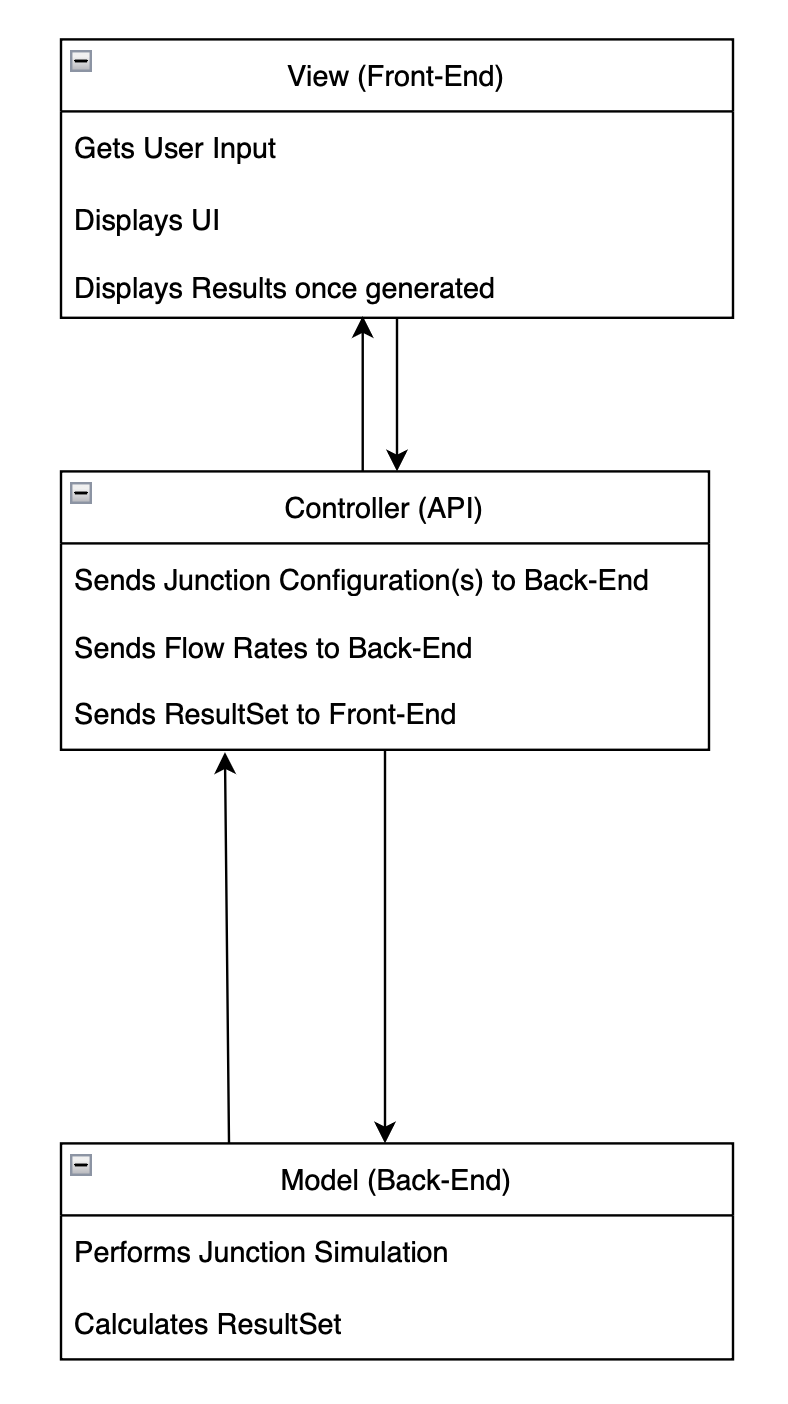
\includegraphics[width=0.5\textwidth]{pattern.png}
    \caption{MVC Pattern}
    \label{pattern}
\end{figure}

Using the MVC pattern will aid us in separating concerns, making the software more modular and easier to maintain. It will also help us separate the development responsibilities between the team members, with some working on the front-end, some on the back-end and some on the API.

\section{Front-End}
%Discussion of using Python and Pygame/similar libraries to create the user interface (including parsing user input) and graphics
For the front-end, we have decided to use Python and the PyQT toolkit to create the user interface. This is because the whole group is familiar 
with the frameworks, and it is a powerful and flexible toolkit that will allow us to create a user-friendly interface.

\subsection{User Interface}
The user interface is structured into three main sections: input configuration, simulation
control, and results display, ensuring a logical workflow from data entry to simulation
analysis. The design prioritises usability, providing clear input options, intuitive controls, and
meaningful output visualisations. The figure below shows a rough mock up of the design we intend to use.


\begin{figure}[H]
    \centering
    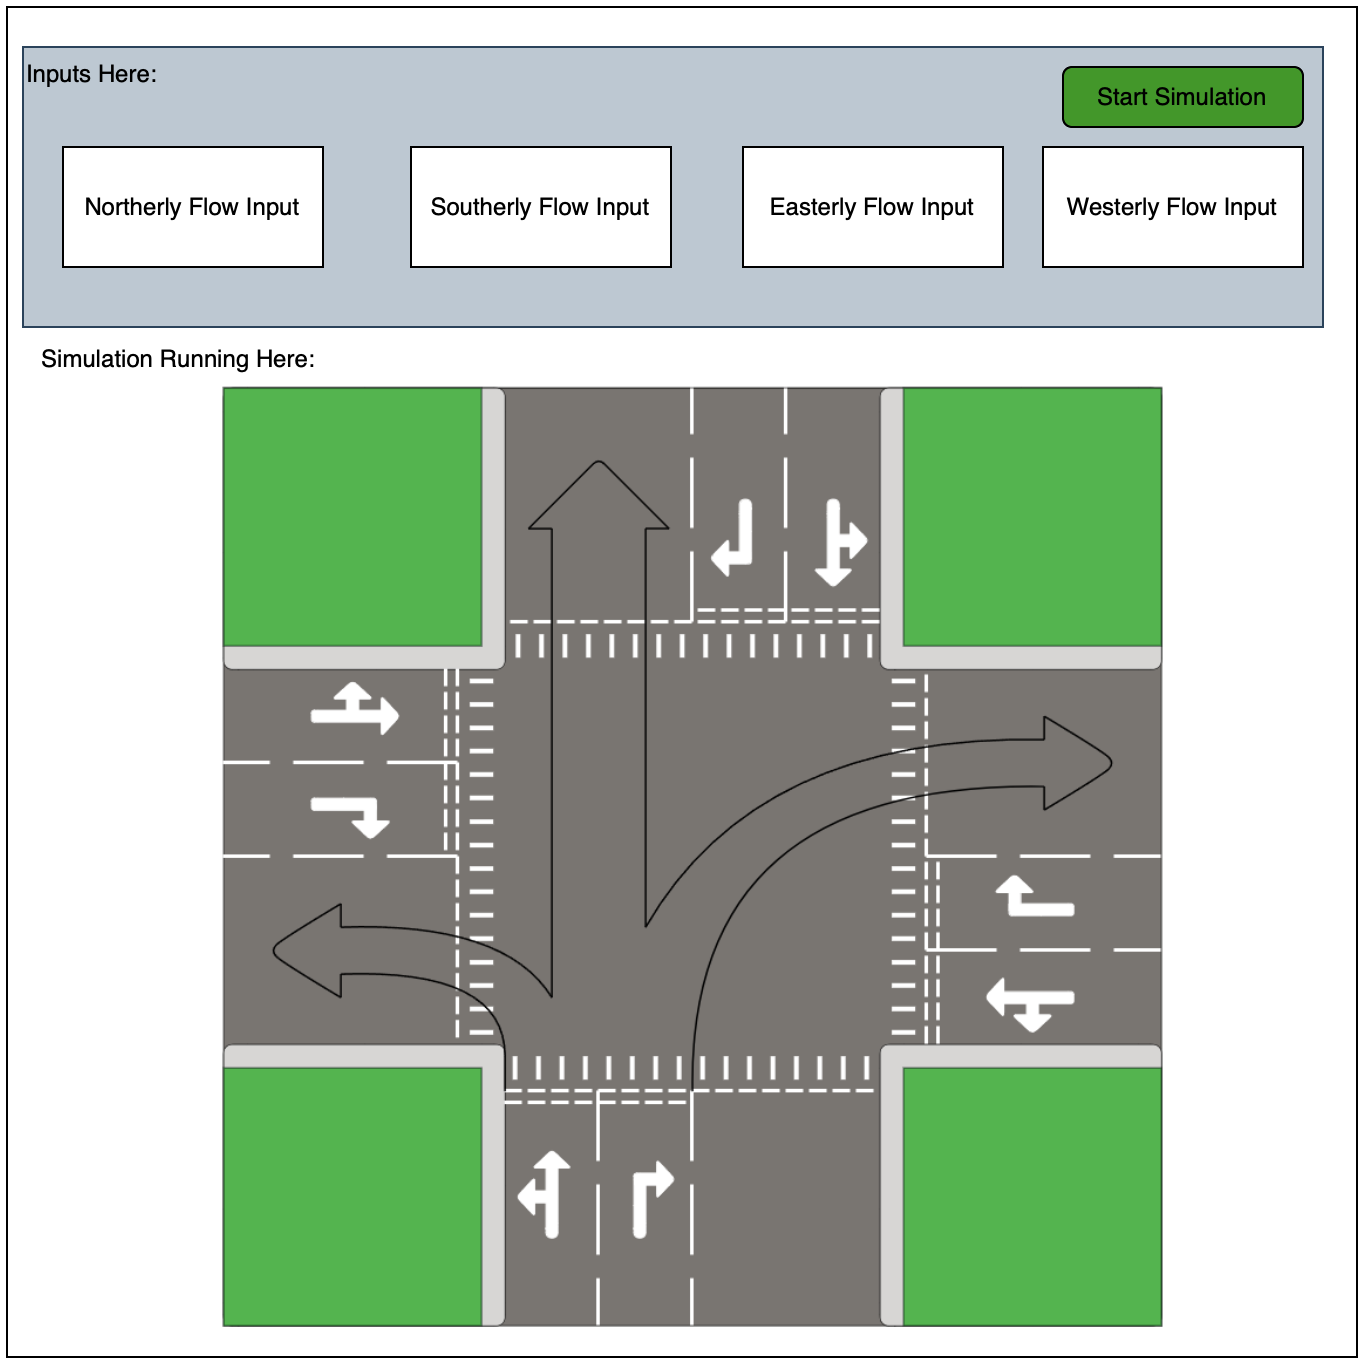
\includegraphics[width=0.8\textwidth]{frontendUI.png}
    \caption{Mock-up of the User Interface}
    \label{frontendUI}
\end{figure}

The user will be able to switch between two tabs on the left-hand side where one tab requires the user to input the traffic flow rates for each exit. The second tab allows the user to change configurable parameters, such as being able to change the number of lanes on each road. Additional
configuration options include checkboxes and radio buttons to enable or disable specific junction features such as left-turn lanes, bus/cycle lanes, and pedestrian crossings. A priority selection system (0 to 4 scale) allows users to define which traffic flows receive higher priority. To improve accessibility and ease of use, tooltips and help text will guide users in configuring their simulation parameters correctly.

\subsection{Simulation Control/Interfacing with Back-End}
The simulation control section includes essential interactive buttons for managing the
simulation process. The "Run Simulation" button will validate the input to ensure that it is within the required range and that there are no conflicts between certain parameters before sending the user-defined inputs to the back-end
for processing. Afterwards, the back-end will run the simulation and to return the results to the front-end when it is done processing. 
The "Reset" button allows users to clear all inputs and reconfigure the
junction settings. A progress indicator provides real-time feedback, notifying users when the
simulation is running to prevent duplicate submissions and improve overall responsiveness.

\subsection{Integration with Back-End and Data Flow}
The front-end communicates with the Python-based backend to process inputs and retrieve simulation results. The data flow follows:
\begin{enumerate}
    \item Users input traffic parameters and configure junction settings.
    \item The front-end validates inputs to prevent errors.
    \item The validated data is sent to the backend simulation engine for processing.
    \item The backend computes traffic performance metrics, including wait times, queue lengths, and efficiency scores.
    \item The results are returned to the front-end, which displays them in structured tables, charts, and animations.
\end{enumerate}

The front-end will also use PyQt’s 2D animation capabilities to provide a visual
representation of traffic flow, simulating vehicle movement, queue formation, and signal
changes dynamically. Since both the front-end and backend are developed in Python,
integration is seamless, using direct function calls instead of external APIs.

\subsection{Error Handling (User)}
Throughout the whole process of the software, from inputting the parameters to displaying the results, the front-end will have error handling to ensure that the software is robust and reliable.
Friendly error messages will be displayed to the user if they input invalid parameters or if there is an error in the simulation. For repeated invalid inputs, the system will provide progressive guidance to users rather
than displaying generic error messages. Where possible, minor formatting issues will be
auto-corrected or users will be prompted with suggested values. For example, if a negative
vehicle flow rate is entered, the system will either convert it to a positive value or display a
clear explanation prompting re-entry. The following pictures show examples of error messages that will be displayed:

\begin{figure}[H]
    \centering
    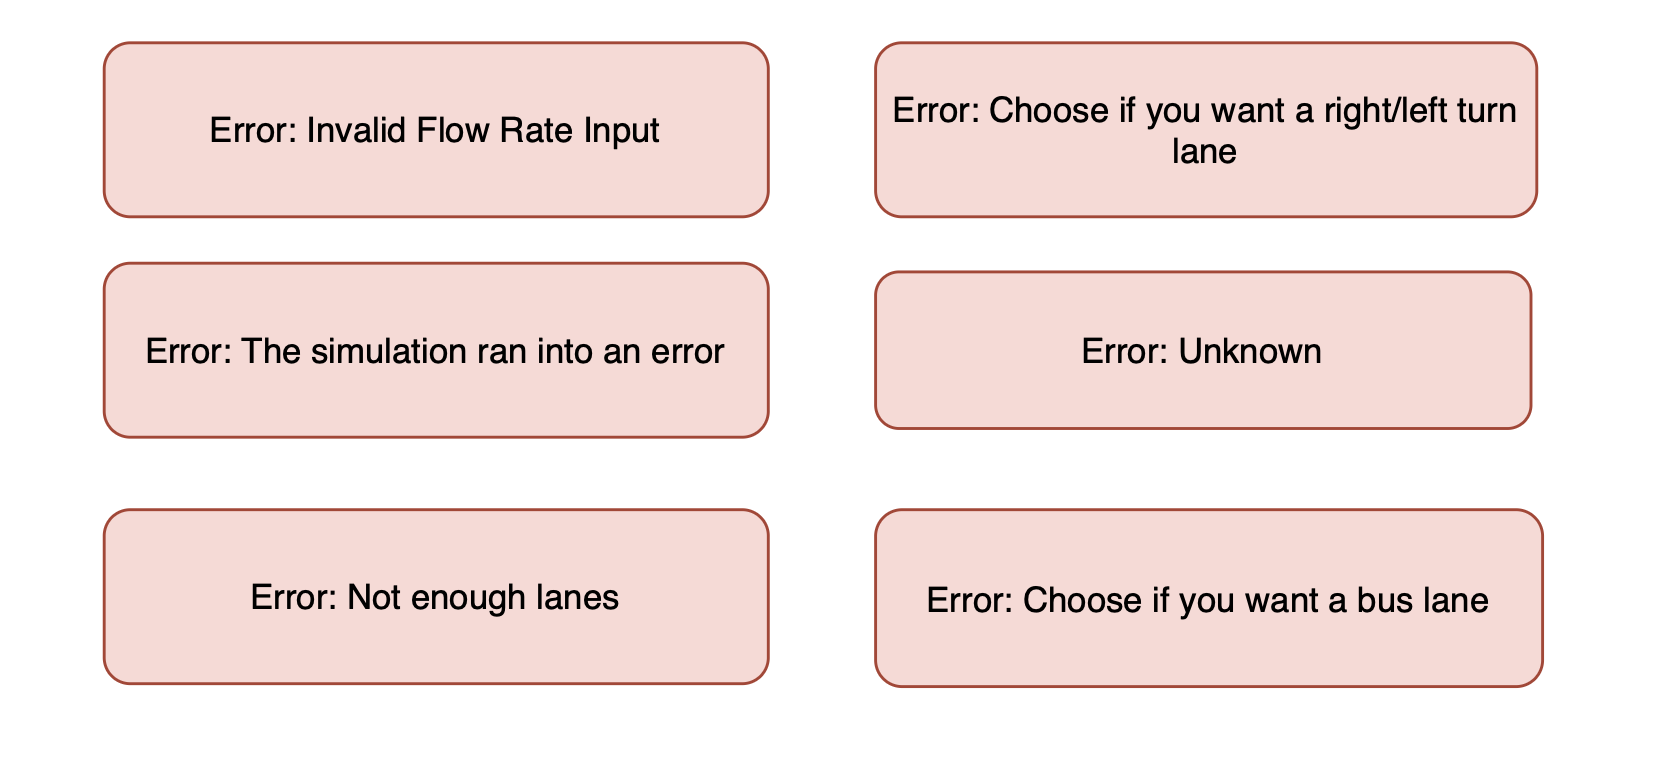
\includegraphics[width=\textwidth]{errormsg.png}
    \caption{Examples of Error Messages}
    \label{errormsg}
\end{figure}

\subsection{Error Handling (Developers)}
To enhance maintainability and debugging efficiency, the front-end will incorporate an error
logging mechanism. When an issue arises—such as invalid input, backend failure, or
unexpected UI behaviour—the system will log the error details into a local log file. This log
will include timestamps, error descriptions, and system state information, allowing
developers to diagnose and resolve issues efficiently.

\section{Back-End}
%Discussion of the design of the simulation
For the back-end, we have decided to implement it in Python due to the whole group being familiar with the language, and to make 
interfacing between the front-end and back-end simple. 

\subsection{Simulation}

We plan to use objects to simulate the junction configurations and calculate 
the junction efficiency metrics and overall scores, with the structure of classes being as follows:

\begin{figure}[H]
    \centering
    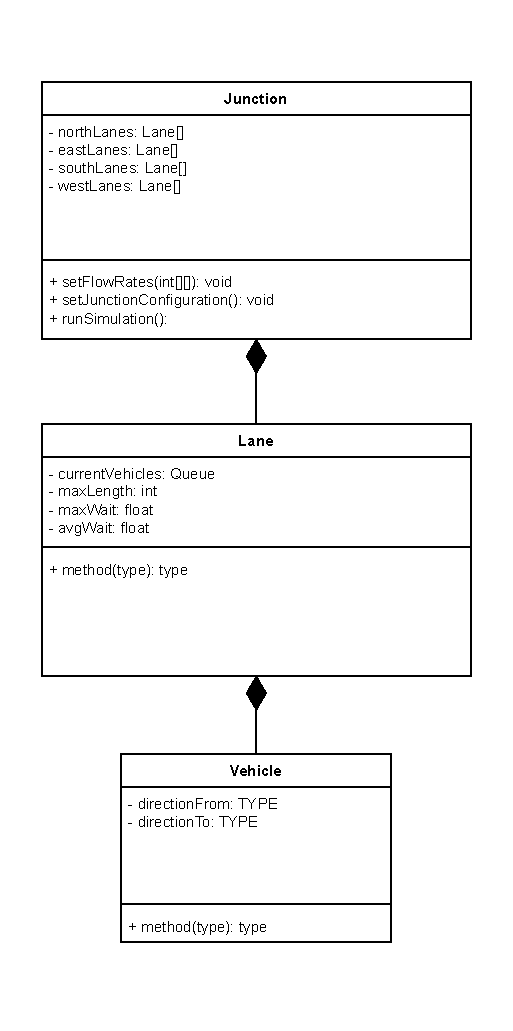
\includegraphics[width=0.8\textwidth]{JunctionSimulationClassDiagram.drawio.pdf}
    \caption{Junction Simulation Class Diagram}
    \label{class diagram}
\end{figure}

The Junction class contains four Direction objects, each representing a road entering the junction. Each of these Direction 
objects contain an array of Lane objects, representing each lane of the road. To set up the simulation, the front-end will 
call two functions: `setFlowRates` to set the flow rates from each direction to the other directions, passed in the form of 
a `FlowRates` object, and `setJunctionConfiguration` to set the specific settings of the junction (e.g. is there a left turn 
lane, how many lanes there are on each incoming road) passed in the form of a Parameters object. For each junction configuration 
generated by the user, a Junction object will be created and be passed a Parameters object corresponding to those configuration 
settings. We decided to use objects for passing the data instead of passing each setting as an individual parameter 
(`setJunctionConfiguration`) or passing the flow rates as a 2D-array (`setFlowRates`) since objects would be easier to work with 
(for example, no scope for miscommunication about what the indices represent) and make it easier to extend the capabilities of 
the software in the future.

When `runSimulation` is run, a for loop will iterate for a set number of iterations (to be decided during development), during 
which it will choose the most optimal state for the traffic lights (in terms of traffic flow) based on the previous state and the 
traffic sequencing priorities, as well as call `simulateUpdate` for each Direction object, to add and remove Vehicle objects from 
its Lane objects to simulate vehicles waiting to transit and transiting the junction. After all the iterations, it will call for 
the junction efficiency metrics of each direction using `getMaxLength()`, `getMaxWait()`, and `getAvgWait()`, calculate the 
overall score for the configuration, and then instantiate a ResultSet object with the metrics and score to return to the front-end.

Each Direction object has a dictionary called `pools`, with the key being the direction vehicles would like to exit to (represented 
in the code with an Enum) and the value being the number of cars that have arrived at the junction that want to exit in that 
direction. Each `Lane` has a limit on the number of vehicles it can contain (`queueLimit`), and at each call of `simulateUpdate`, 
vehicles are added to each lane to replace any vehicles which have transited the junction, with their respective `pools` value 
being decreased by the number added to the lane and increased by the corresponding traffic flow rate multiplied by the time the 
iteration represents.

For the traffic lights, we decided that there would be four main states they could be in (ignoring pedestrian crossings): North and 
South traffic allowed to exit left and ahead, North and South traffic allowed to exit right, East and West traffic allowed to exit 
left and ahead, East and West traffic allowed to exit right. This state is passed in the form of an Enum to the Direction and then 
Lane objects via `simulateUpdate`, where a Lane only dequeues Vehicle objects if the `directionFrom` and `directionTo` attributes 
of the current Vehicle agree with the state passed. For the simulation, we have assumed that if two vehicles coming from opposite 
directions are turning right in the junction, they turn in front of each other rather than behind each other.


\subsection{Interfacing with Frontend}
% not using API anymore :(

Even though the frontend and backend portions of the application will be 
written in Python we will make sure to have a quasi API between the two 
different components, encapsulating all logic and intefacing between the 
frontend and backend into functions that would be a 1:1 translation into 
what an API would be capable of. For example simulating a junction's 
performance would only require a single call similar to how it would require 
a single call to an endpoint if this was to expand to use an API.

Separation in this manner will allow for us to keep development efficient, 
allowing those on the frontend to focus on their tasks and those on the 
backend to focus on theirs by keeping a well defined method of interaction 
between the two sides.

If the system was to expand in the future it would be simple to split these 
functions into an API controller and split the front and backend into a 
server and client architecture.

\subsection{Validation and Error handling}

There are a large variety of parameters that can be inputted into the system, it is 
important that they are properly validated, this will be achieved through functions 
that check each of the parameters is in the required range and that there are no 
conflicts between certain parameters. For example the sum of each direction's output 
flows must be equal to the inflow as well as the requirement for each flow to be 
greater than or equal to 0. 

We will use automated testing to check that the system validates sets of input 
parameters correctly on each build, any changes to the validation code will be then 
checked automatically that they produce the correct result. 

As we are using python for parts of the project and they are going to live 
in the same project we will be able to reuse the validation logic between both 
sections, guaranteeing consistent behaviour. This also means that if the system 
is expanded in the future it would allow for quick and consistent changes to the 
validation logic across the whole application.

\section{Deployment}
%This is where we discuss containerisation
As we will be programming both the frontend and backend in python under a single 
application we will package for each operating system separately, this will require 
a build process for each platform. As we are developing and testing across all of 
our team members personal computers we will effectively be testing along the way 
if it works well across all platforms. We have 2 Mac, 3 Windows and 1 Linux machine.

\subsection{Modularity}
Despite our team forgoing the descision to create a separate frontend and backend 
service we will still make sure that there is a degree of separation between the 
two, all the logic will be kept to itself and not intertwined inside the frontend.

This will allow us to expand easily in the future by eschewing the backend into 
it's own service with the front end clients being swapped in and out and tailored 
to individual customer's needs. This backend service could be containerised, this 
would allow for it to be setup in a distributed network not only for greater 
perfomance but also fault tolerance and reliability.

Docker/Podman is an open standard and would allow for these containers to be ran 
on any platform with a container engine.

\subsection{Scalability and Fault tolerance}
In the future the backend could be made quite simply into a basic docker container, 
allowing it to be deployed on any linux machine with great devops ergonomics. In the 
initial prototype stage that we will submit the system will be running locally on the 
user's machine, if any non fixable faults are encountered the system will simply 
restart with an error message, for any fixable faults it will allow the user to change 
whatever the causing parameter was.

Usage of containerisation in this manner would allow us to scale the system as the 
needs of it grow, if for example we have multiple applications taking data from the 
backend at a time we can run multiple instances of the backend and use a load balancer 
to distribute client calls between each instance. If the client requires a higher level 
of uptime than a single instance allows, If they need fault tolerance than a single 
geographic location and instance allows then this would be simple to achieve using a 
set of containers in a distributed network.

Developing inside a container allows for a consistent build and deployment environment 
every time, if a client has an installation of docker/podman then they would be able to 
run the software just as they would any other container. Containers are largely similar 
to bare metal performance would have minimal effect on an app like this especially as 
we wouldn't have much interaction with the underlying system e.g filesystem.

\end{document}
